\begin{figure}[ht]\label{fig:preorder}
\begin{center}


\tikzset{every picture/.style={line width=0.75pt}} %set default line width to 0.75pt        

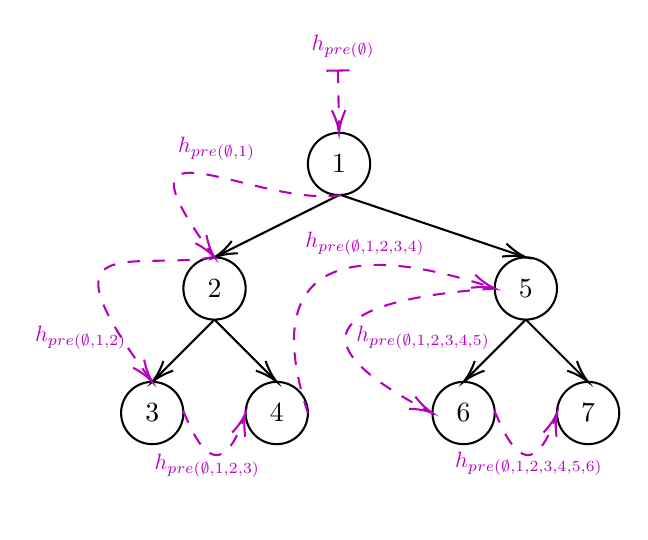
\begin{tikzpicture}[x=0.75pt,y=0.75pt,yscale=-1,xscale=1]
%uncomment if require: \path (0,247.3125); %set diagram left start at 0, and has height of 247.3125

%Shape: Circle [id:dp5747539528933221] 
\draw   (150,75) .. controls (150,66.72) and (156.72,60) .. (165,60) .. controls (173.28,60) and (180,66.72) .. (180,75) .. controls (180,83.28) and (173.28,90) .. (165,90) .. controls (156.72,90) and (150,83.28) .. (150,75) -- cycle ;
%Shape: Circle [id:dp6584741963271383] 
\draw   (90,135) .. controls (90,126.72) and (96.72,120) .. (105,120) .. controls (113.28,120) and (120,126.72) .. (120,135) .. controls (120,143.28) and (113.28,150) .. (105,150) .. controls (96.72,150) and (90,143.28) .. (90,135) -- cycle ;
%Shape: Circle [id:dp42608384351679063] 
\draw   (240,135) .. controls (240,126.72) and (246.72,120) .. (255,120) .. controls (263.28,120) and (270,126.72) .. (270,135) .. controls (270,143.28) and (263.28,150) .. (255,150) .. controls (246.72,150) and (240,143.28) .. (240,135) -- cycle ;
%Shape: Circle [id:dp4039562507165959] 
\draw   (60,195) .. controls (60,186.72) and (66.72,180) .. (75,180) .. controls (83.28,180) and (90,186.72) .. (90,195) .. controls (90,203.28) and (83.28,210) .. (75,210) .. controls (66.72,210) and (60,203.28) .. (60,195) -- cycle ;
%Shape: Circle [id:dp6061665496522999] 
\draw   (120,195) .. controls (120,186.72) and (126.72,180) .. (135,180) .. controls (143.28,180) and (150,186.72) .. (150,195) .. controls (150,203.28) and (143.28,210) .. (135,210) .. controls (126.72,210) and (120,203.28) .. (120,195) -- cycle ;
%Straight Lines [id:da040054788995673274] 
\draw    (165,90) -- (106.79,119.11) ;
\draw [shift={(105,120)}, rotate = 333.43] [color={rgb, 255:red, 0; green, 0; blue, 0 }  ][line width=0.75]    (10.93,-3.29) .. controls (6.95,-1.4) and (3.31,-0.3) .. (0,0) .. controls (3.31,0.3) and (6.95,1.4) .. (10.93,3.29)   ;

%Straight Lines [id:da9417356343431731] 
\draw    (166,90) -- (253.1,119.36) ;
\draw [shift={(255,120)}, rotate = 198.63] [color={rgb, 255:red, 0; green, 0; blue, 0 }  ][line width=0.75]    (10.93,-3.29) .. controls (6.95,-1.4) and (3.31,-0.3) .. (0,0) .. controls (3.31,0.3) and (6.95,1.4) .. (10.93,3.29)   ;

%Straight Lines [id:da7471003825026084] 
\draw    (105,150) -- (76.41,178.59) ;
\draw [shift={(75,180)}, rotate = 315] [color={rgb, 255:red, 0; green, 0; blue, 0 }  ][line width=0.75]    (10.93,-3.29) .. controls (6.95,-1.4) and (3.31,-0.3) .. (0,0) .. controls (3.31,0.3) and (6.95,1.4) .. (10.93,3.29)   ;

%Straight Lines [id:da3919517743443004] 
\draw    (105,150) -- (133.59,178.59) ;
\draw [shift={(135,180)}, rotate = 225] [color={rgb, 255:red, 0; green, 0; blue, 0 }  ][line width=0.75]    (10.93,-3.29) .. controls (6.95,-1.4) and (3.31,-0.3) .. (0,0) .. controls (3.31,0.3) and (6.95,1.4) .. (10.93,3.29)   ;

%Shape: Circle [id:dp09204588637656741] 
\draw   (210,195) .. controls (210,186.72) and (216.72,180) .. (225,180) .. controls (233.28,180) and (240,186.72) .. (240,195) .. controls (240,203.28) and (233.28,210) .. (225,210) .. controls (216.72,210) and (210,203.28) .. (210,195) -- cycle ;
%Shape: Circle [id:dp4405799901518632] 
\draw   (270,195) .. controls (270,186.72) and (276.72,180) .. (285,180) .. controls (293.28,180) and (300,186.72) .. (300,195) .. controls (300,203.28) and (293.28,210) .. (285,210) .. controls (276.72,210) and (270,203.28) .. (270,195) -- cycle ;
%Straight Lines [id:da9350681939269714] 
\draw    (255,150) -- (226.41,178.59) ;
\draw [shift={(225,180)}, rotate = 315] [color={rgb, 255:red, 0; green, 0; blue, 0 }  ][line width=0.75]    (10.93,-3.29) .. controls (6.95,-1.4) and (3.31,-0.3) .. (0,0) .. controls (3.31,0.3) and (6.95,1.4) .. (10.93,3.29)   ;

%Straight Lines [id:da6947341181570368] 
\draw    (255,150) -- (283.59,178.59) ;
\draw [shift={(285,180)}, rotate = 225] [color={rgb, 255:red, 0; green, 0; blue, 0 }  ][line width=0.75]    (10.93,-3.29) .. controls (6.95,-1.4) and (3.31,-0.3) .. (0,0) .. controls (3.31,0.3) and (6.95,1.4) .. (10.93,3.29)   ;

%Curve Lines [id:da39887266209810046] 
\draw [color={rgb, 255:red, 182; green, 0; blue, 192 }  ,draw opacity=1 ] [dash pattern={on 4.5pt off 4.5pt}]  (166,90) .. controls (124.21,96.28) and (50.74,46.81) .. (104.18,118.9) ;
\draw [shift={(105,120)}, rotate = 233.26] [color={rgb, 255:red, 182; green, 0; blue, 192 }  ,draw opacity=1 ][line width=0.75]    (10.93,-3.29) .. controls (6.95,-1.4) and (3.31,-0.3) .. (0,0) .. controls (3.31,0.3) and (6.95,1.4) .. (10.93,3.29)   ;

%Curve Lines [id:da20716783829208452] 
\draw [color={rgb, 255:red, 182; green, 0; blue, 192 }  ,draw opacity=1 ] [dash pattern={on 4.5pt off 4.5pt}]  (105,120) .. controls (63.21,126.28) and (20.43,106.51) .. (74.18,178.9) ;
\draw [shift={(75,180)}, rotate = 233.26] [color={rgb, 255:red, 182; green, 0; blue, 192 }  ,draw opacity=1 ][line width=0.75]    (10.93,-3.29) .. controls (6.95,-1.4) and (3.31,-0.3) .. (0,0) .. controls (3.31,0.3) and (6.95,1.4) .. (10.93,3.29)   ;

%Curve Lines [id:da03343755971007978] 
\draw [color={rgb, 255:red, 182; green, 0; blue, 192 }  ,draw opacity=1 ] [dash pattern={on 4.5pt off 4.5pt}]  (150,195) .. controls (124.63,117.7) and (174.99,113.35) .. (239.03,134.68) ;
\draw [shift={(240,135)}, rotate = 198.57999999999998] [color={rgb, 255:red, 182; green, 0; blue, 192 }  ,draw opacity=1 ][line width=0.75]    (10.93,-3.29) .. controls (6.95,-1.4) and (3.31,-0.3) .. (0,0) .. controls (3.31,0.3) and (6.95,1.4) .. (10.93,3.29)   ;

%Curve Lines [id:da25925997339396334] 
\draw [color={rgb, 255:red, 182; green, 0; blue, 192 }  ,draw opacity=1 ] [dash pattern={on 4.5pt off 4.5pt}]  (240,135) .. controls (177.81,139.29) and (130.97,154.16) .. (208.82,194.39) ;
\draw [shift={(210,195)}, rotate = 207.1] [color={rgb, 255:red, 182; green, 0; blue, 192 }  ,draw opacity=1 ][line width=0.75]    (10.93,-3.29) .. controls (6.95,-1.4) and (3.31,-0.3) .. (0,0) .. controls (3.31,0.3) and (6.95,1.4) .. (10.93,3.29)   ;

%Curve Lines [id:da04019975701917122] 
\draw [color={rgb, 255:red, 182; green, 0; blue, 192 }  ,draw opacity=1 ] [dash pattern={on 4.5pt off 4.5pt}]  (240,195) .. controls (239.51,189.37) and (254.2,242.24) .. (269.54,196.42) ;
\draw [shift={(270,195)}, rotate = 467.79] [color={rgb, 255:red, 182; green, 0; blue, 192 }  ,draw opacity=1 ][line width=0.75]    (10.93,-3.29) .. controls (6.95,-1.4) and (3.31,-0.3) .. (0,0) .. controls (3.31,0.3) and (6.95,1.4) .. (10.93,3.29)   ;

%Straight Lines [id:da47300784385513417] 
\draw [color={rgb, 255:red, 182; green, 0; blue, 192 }  ,draw opacity=1 ] [dash pattern={on 4.5pt off 4.5pt}]  (164.5,30) -- (164.97,58) ;
\draw [shift={(165,60)}, rotate = 269.05] [color={rgb, 255:red, 182; green, 0; blue, 192 }  ,draw opacity=1 ][line width=0.75]    (10.93,-3.29) .. controls (6.95,-1.4) and (3.31,-0.3) .. (0,0) .. controls (3.31,0.3) and (6.95,1.4) .. (10.93,3.29)   ;
\draw [shift={(164.5,30)}, rotate = 269.05] [color={rgb, 255:red, 182; green, 0; blue, 192 }  ,draw opacity=1 ][line width=0.75]    (0,5.59) -- (0,-5.59)   ;
%Curve Lines [id:da4854965313512276] 
\draw [color={rgb, 255:red, 182; green, 0; blue, 192 }  ,draw opacity=1 ] [dash pattern={on 4.5pt off 4.5pt}]  (90,195) .. controls (89.51,189.37) and (104.2,242.24) .. (119.54,196.42) ;
\draw [shift={(120,195)}, rotate = 467.79] [color={rgb, 255:red, 182; green, 0; blue, 192 }  ,draw opacity=1 ][line width=0.75]    (10.93,-3.29) .. controls (6.95,-1.4) and (3.31,-0.3) .. (0,0) .. controls (3.31,0.3) and (6.95,1.4) .. (10.93,3.29)   ;


% Text Node
\draw (165,75) node  [align=left] {1};
% Text Node
\draw (105,135) node  [align=left] {2};
% Text Node
\draw (255,135) node  [align=left] {5};
% Text Node
\draw (120,138) node  [align=left] {$ $};
% Text Node
\draw (75,195) node  [align=left] {3};
% Text Node
\draw (135,195) node  [align=left] {4};
% Text Node
\draw (225,195) node  [align=left] {6};
% Text Node
\draw (285,195) node  [align=left] {7};
% Text Node
\draw (167,18.5) node [scale=0.8,color={rgb, 255:red, 182; green, 0; blue, 192 }  ,opacity=1 ] [align=left] {$\displaystyle h_{pre( \emptyset )}$};
% Text Node
\draw (106,67.5) node [scale=0.8,color={rgb, 255:red, 182; green, 0; blue, 192 }  ,opacity=1 ] [align=left] {$\displaystyle h_{pre( \emptyset ,1)}$};
% Text Node
\draw (40.5,158.5) node [scale=0.8,color={rgb, 255:red, 182; green, 0; blue, 192 }  ,opacity=1 ] [align=left] {$\displaystyle h_{pre( \emptyset ,1,2)}$};
% Text Node
\draw (101.5,220.5) node [scale=0.8,color={rgb, 255:red, 182; green, 0; blue, 192 }  ,opacity=1 ] [align=left] {$\displaystyle h_{pre( \emptyset ,1,2,3)}$};
% Text Node
\draw (177.5,113.5) node [scale=0.8,color={rgb, 255:red, 182; green, 0; blue, 192 }  ,opacity=1 ] [align=left] {$\displaystyle h_{pre( \emptyset ,1,2,3,4)}$};
% Text Node
\draw (205.5,158.5) node [scale=0.8,color={rgb, 255:red, 182; green, 0; blue, 192 }  ,opacity=1 ] [align=left] {$\displaystyle h_{pre( \emptyset ,1,2,3,4,5)}$};
% Text Node
\draw (256.5,219.5) node [scale=0.8,color={rgb, 255:red, 182; green, 0; blue, 192 }  ,opacity=1 ] [align=left] {$\displaystyle h_{pre( \emptyset ,1,2,3,4,5,6)}$};


\end{tikzpicture}

\end{center}
\caption{Preorder}
\end{figure}
